\documentclass[onecolumn,final]{ltugboat}

%% Notes to the editor
%% -------------------
%% 1. LuaTeX is required to compile this article.
%% 2. Following fonts are required:
%% 2.1. RIT Rachana (https:/rachana.org.in)
%% 3. The fonts directory has required fonts.
%% 

% \usepackage[p]{rit-doc}
 \usepackage[w,doc]{rit-doc}
\usepackage{ragged2e,makecell,shortvrb,array,multirow}
\MakeShortVerb{\|}
\usepackage{microtype}
\usepackage{unicodefonttable}

\makeatletter
\newenvironment{exbox}[1][-\listparindent]
  {\par\smallskip\hspace*{#1}}
  {\par\smallskip}
\newdimen\xmpwd
\newdimen\lshift
\if@twocolumn
  \setlength\xmpwd{\dimexpr(\linewidth+1.75\leftmargin)}
  \setlength\lshift{-2.5\leftmargin}
\else
  \setlength\xmpwd{.6\linewidth}
  \setlength\lshift{-\listparindent}
\fi
\setcounter{bottomnumber}{2}
\setcounter{topnumber}{4}
\def\sectionautorefname{Section}
\def\subsectionautorefname{Section}
\def\subsubsectionautorefname{Section}
\def\tsm{\small}
\def\pdf{\PDF\xspace}
\def\cmap{{\tsm CM}ap\xspace}
\def\rit{{\tsm RIT}\xspace}
\def\otf{{\tsm OTF}\xspace}
\def\ttf{{\tsm TTF}\xspace}
\def\woff{{\tsm WOFF2}\xspace}
\def\ofl{{\tsm OFL}\xspace}
\def\ctan{\CTAN\xspace}

\makeatother

\begin{document}

\setcounter{page}{1}

\title{Fonts in Malayalam script by Rachana Institute of Typography}

\author{C.\,V.~Radhakrishnan}
\netaddress{cvr(at)river-valley(dot)org}
\ORCID{0000-0001-7511-2910}
\address{River Valley Technologies, River Valley Campus, Malayinkeezh,
  Trivandrum 695571, India} 
\personalURL{http://river-valley.com}

\author{K.\,V.~Rajeesh}
\address{Rachana Institute of Typography}
\netaddress{rajeesh(at)rachana(dot)org(dot)in} 
\personalURL{https://rachana.org.in/}

\author{K.\,H.~Hussain}
\address{Rachana Institute of Typography}
\netaddress{hussain(at)rachana(dot)org(dot)in} 
\personalURL{https://rachana.org.in/}

\maketitle

\begin{abstract}
  This article describes about all the fonts published by Rachana
  Institute of Typography (\rit), a not-for-profit organization, engaged
  in developing, publishing and promoting OpenType fonts under
  the terms of Open Fonts License.  It further tells about the
  \LaTeX{} package, |rit-fonts.sty| that accompanies the bundle of
  \rit fonts released at \CTAN.
\end{abstract}

\section{The background}

The \rit is a not-for-profitprofit digital foundry in Kerala, India,
that had released ten families of Indic script fonts in different
formats---\otf, \ttf, \woff under the terms of Open Font License
(\ofl) \cite{ofl}.  The following are the technical objectives behind
the setting up of \rit:
\begin{enumerate}
\item to resurrect the original script of Malayalam that was diluted
  by dropping hundreds of conjuncts and ligatures when reformed script
  for the language was introduced by the government of Kerala to fit
  the keyboad of typewriters.
\item to develop fonts that completely adhere to the definitive
  character set prevalent through ages.
\item to completely revamp the OpenType layout {\tsm (GSUB)} of \rit
  fonts to uphold the right spirit of comprehensive character set and
  to replace all previous modifications.
\item to redesign all the glyphs in the flagship font, \rit Rachana.
\item to freshly redesign \rit Rachana Italic, Bold and BoldItalic and
  to generate respective font variants.
\item to encourage the usage of code-driven font development models by
  employing character description languages like \MF\ and \MP.
\end{enumerate}

\section{The \rit fonts}

The \rit has published the following fonts till date by striving to
meet the aforesaid objectives :
\begin{description}
\item[Serif] \mbox{}
  \begin{enumerate}
  \item \rit Rachana (regular, bold, italic, bold-italic)
  \begin{exbox}[\lshift]
    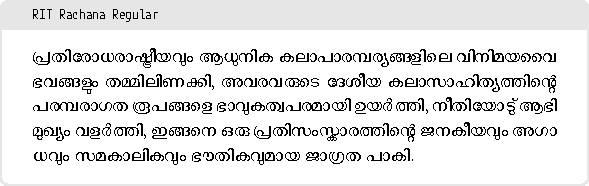
\includegraphics[width=\xmpwd,page=1]{font-example.pdf}
  \end{exbox}
  \item \rit Panamana (regular)
  \begin{exbox}[\lshift]
    \includegraphics[width=\xmpwd,page=2]{font-example.pdf}
  \end{exbox}
  \end{enumerate}
\item[Sans-serif] \mbox{}\par
  \begin{enumerate}
  \item \rit MeeraNew (regular)
  \begin{exbox}[\lshift]
    \includegraphics[width=\xmpwd,page=3]{font-example.pdf}
  \end{exbox}
  \item \rit TN Joy (regular, bold, extra-bold)
  \begin{exbox}[\lshift]
    \includegraphics[width=\xmpwd,page=4]{font-example.pdf}
  \end{exbox}
  \end{enumerate}
\item[Display] \mbox{}\par
  \begin{enumerate}
  \item \rit Keraleeyam (regular, italic)
  \item \rit Sundar (regular)
  \item \rit Uroob (regular)
  \item \rit Karuna (regular)
  \item \rit Chingam (regular)
  \end{enumerate}
\item[Handwriting] \mbox{}\par
  \begin{enumerate}
  \item \rit Ezhuthu (regular)
  \item \rit Kutty (regular)
  \end{enumerate}
\end{description}
The font samples of display and handwriting fonts and the variants of
serif and sans-serif fonts are available separately, see
\cite{font-samples}.

\section{The package, \texttt{rit-fonts.sty}} \label{sec:rit-fonts}

The package, |rit-fonts.sty| has been developed to assist seamless
usage of the fonts in \LaTeX{} documents. The package needs
|fontspec.sty| (to load the fonts and to access OpenType font
features) and |polyglossia| (for language switching and hyphernation)
\cite{fontspec,polyglossia}, both these packages are available in any
standard \TeX\ distribution.  The fonts become accessible to the
typesetting engine employed when you load the package with the
following command:

\begin{lstlisting}[xleftmargin=1.5\leftmargin]
  \usepackage[...options...]{rit-fonts}
\end{lstlisting}

\subsection{The options}

The package has the following options:
\begin{description}[itemsep=6pt]
\item[path] specify the location of fonts, if the user prefers to keep
  the fonts in a custom path, the default being |empty|. 
\begin{lstlisting}[xleftmargin=\leftmargin]
  \usepackage[path=./ml-fonts/,<options>]{rit-fonts}
\end{lstlisting}
  The usage of |path| option will look like above, if you keep the
  \rit fonts in a subdirectory by name, |./ml-fonts/|, in your working
  directory.
  
\item[extn] specify the extension of fonts, if the user prefers to use
  a specific font format like |.otf| or |.ttf|, default being |.ttf|.
\begin{lstlisting}[xleftmargin=\leftmargin]
  \usepackage[extn=.otf,<options>]{rit-fonts}
\end{lstlisting}

\item[RM] set the |\rmdefault| by providing the font name.
\begin{lstlisting}[xleftmargin=\leftmargin]
  \usepackage[RM=RIT-Rachana,<options>]{rit-fonts}
\end{lstlisting}
  \rit-Rachana will be set as the default |\rmfamily| font.

\item[SF] set the |\sfdefault| by providing the font name.
\begin{lstlisting}[xleftmargin=\leftmargin]
  \usepackage[SF=RIT-MeeraNew,<options>]{rit-fonts}
\end{lstlisting}
  \rit MeeraNew will be set as the default |\sffamily| font.

\item[ScaleRM] scale the |\rmdefault| font by providing the value.
\begin{lstlisting}[xleftmargin=\leftmargin]
  \usepackage[ScaleRM=1.5,<options>]{rit-fonts}
\end{lstlisting}
  The default value is |1|.  Assuming that we have chosen |RIT Rachana| as
  the |\rmdefault|, then by applying |Scale=1.5|, we get,
  \begin{exbox}
    \includegraphics[width=\xmpwd,page=5]{font-example.pdf}
  \end{exbox}

\item[ScaleSF] scale the |\sfdefault| font by providing the value.
\begin{lstlisting}[xleftmargin=\leftmargin]
  \usepackage[ScaleSF=.8,<options>]{rit-fonts}
\end{lstlisting}
  The default value is |1|.

\item[ScaleDS, ScaleHW] as in the previous cases, scale factor can be provided
  for display and handwriting fonts respectively. The value of
  |ScaleDS| applies to the fonts categorized as |Display| fonts while
  that of |ScaleHW| applies to |RIT Ezhuthu| and |RIT Kutty| fonts. 

\item[osf, oldstyle] uses |oldstyle| numbers, if the font has oldstyle
  numbers available. In this bundle of fonts, only \rit Rachana has
  oldstyle numbers.
  \medskip

  \begin{exbox}
    \includegraphics[width=\xmpwd,page=6]{font-example.pdf}
  \end{exbox}

\item[lf, lining] this is the default style of numbers in all the
  fonts.

\item[df] add more font features available in |fontspec| package that
  you want to add to the |\defaultfontfeatures|.
\end{description}

Further, individual fonts can be tailored to suit the user requirement
by making use of |\defaultfontfeatures+| command which will append the
features to the defaults. The usage shall be:
\begin{lstlisting}[xleftmargin=\leftmargin]
\defaultfontfeatures+{<font name>}{<font features>}
\end{lstlisting}

Various {\tsm NFSS} commands like |\fontsize{..}{...}\selectfont|,
|\bfseries|, |\itshape|, |\upshape|, |\scshape|, etc., will work
seamlessly.  For more information on various font features provided by
|fontspec|, kindly go through the package documentation at
\cite{fontspec}.

\section{Sources, downloads and license}

\begin{enumerate}
\item The sources of all the fonts, font making scripts, shaping
  features, kern tables, etc., are available at
  \url{https://gitlab.com/rit-fonts/}. 
\item All the fonts can be downloaded by visiting the \rit website:
  \url{https://rachana.org.in/downloads.html}.
\item All the fonts are shared under the terms of Open Font License
  (\url{https://scripts.sil.org/ofl}). 
\end{enumerate}

\section{The glyph list}

The entire glyph list of \rit Rachana is provided below by making use
of the package |unicodefonttable| \cite{unicodefonttable}.  Only the
glyph list of regular variant alone is provided as an example, while
others can be downloaded from the \rit website \cite{rit-home}.

\ifprint
 \displayfonttable[range-end=F033F]{RIT-Rachana-Regular}
\else
 \displayfonttable[range-end=F033F]{RIT-Rachana-Regular}
\fi


\RaggedRight\small
\bibliographystyle{tugboat}
\bibliography{ml}

\makesignature

\end{document}

%%% Local Variables:
%%% mode: latex
%%% TeX-master: t
%%% End:
